\documentclass[tikz, border=12pt]{standalone}
\usepackage[T1]{fontenc}
\usepackage{mathpazo}
\usepackage{amsmath}
\usetikzlibrary{arrows.meta, calc}

\definecolor{stblue}{HTML}{7B97AD}
\definecolor{sage}{HTML}{7A9A7E}
\definecolor{dkbrown}{HTML}{3D3530}
\definecolor{wmgray}{HTML}{7B7067}
\definecolor{cream}{HTML}{F9F6F0}
\definecolor{border}{HTML}{D4C9B8}
\definecolor{terracotta}{HTML}{C47A6A}

\begin{document}
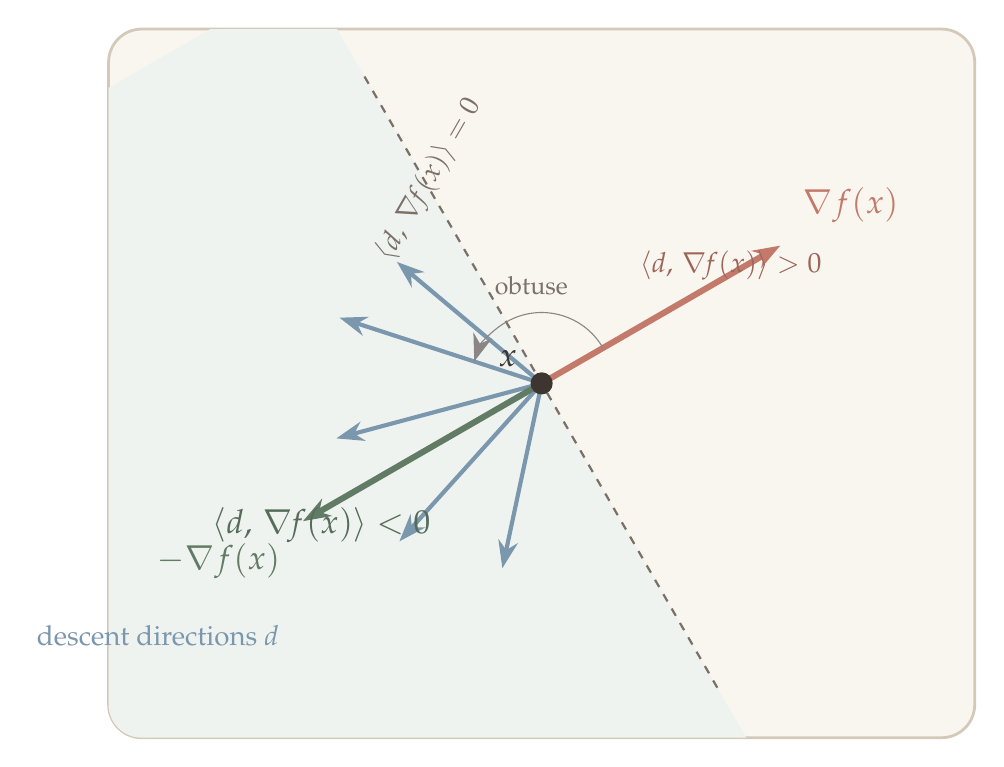
\begin{tikzpicture}[
  >={Stealth[length=3.5mm, width=2.5mm]},
  line width=1.2pt
]

% Background
\fill[cream, rounded corners=12pt] (-5.5,-4.5) rectangle (5.5,4.5);
\draw[border, line width=1pt, rounded corners=12pt] (-5.5,-4.5) rectangle (5.5,4.5);

% ── Half-space shading (descent directions) ──
\begin{scope}
  \clip[rounded corners=12pt] (-5.5,-4.5) rectangle (5.5,4.5);
  \fill[sage!12] (120:6) -- (300:6)
    -- ($(300:6)+(210:12)$) -- ($(120:6)+(210:12)$) -- cycle;
\end{scope}

% ── Boundary line: d^T ∇f(x) = 0 ──
\draw[wmgray, thick, dashed] (120:4.5) -- (300:4.5);

% ── Fan of example descent directions ──
\foreach \a/\r in {140/2.4, 162/2.7, 195/2.7, 228/2.7, 258/2.4} {
  \draw[->, stblue, line width=1.5pt] (0,0) -- (\a:\r);
}

% ── Steepest descent arrow $-\nabla f(x)$ ──
\draw[->, sage!80!black, line width=2.2pt] (0,0) -- (210:3.5);
\node[sage!80!black, font=\large, anchor=north east]
  at ($(210:3.5)+(-0.15,-0.15)$) {$-\nabla f(x)$};

% ── Gradient arrow $\nabla f(x)$ ──
\draw[->, terracotta, line width=2.2pt] (0,0) -- (30:3.5);
\node[terracotta, font=\large, anchor=south west]
  at ($(30:3.5)+(0.15,0.15)$) {$\nabla f(x)$};

% ── Point x ──
\fill[dkbrown] (0,0) circle (4pt);
\node[dkbrown, font=\large, anchor=south east, xshift=-5pt, yshift=2pt]
  at (0,0) {$x$};

% ── Boundary label ──
\node[wmgray, font=\normalsize, rotate=60, anchor=south]
  at ($(120:2.8)+(0.25,0)$) {$\langle d,\, \nabla\!f(x)\rangle = 0$};

% ── Half-space labels ──
\node[sage!70!black, font=\large]
  at (-2.8, -1.8) {$\langle d,\, \nabla\!f(x)\rangle < 0$};
\node[terracotta!70!dkbrown, font=\normalsize]
  at (2.4, 1.5) {$\langle d,\, \nabla\!f(x)\rangle > 0$};

% ── Obtuse angle arc ──
\draw[dkbrown!60, thin, ->] (30:0.9) arc[start angle=30, end angle=162, radius=0.9];
\node[dkbrown!70, font=\small] at (96:1.25) {obtuse};

% ── Descent directions label ──
\node[stblue, font=\normalsize, anchor=east]
  at (-3.2, -3.2) {descent directions $d$};

\end{tikzpicture}
\end{document}
